\newpage
\section{Tuning distance-dependency}

Stepping away, we 




Maybe simplicity of the model makes stuff wrong. Tune to Perin
distance profile.

Let 

In their study, \textcite{Perin2011} heavily rely on a
distance-dependent 


Here we introduce anisotropic networks tuned to reflect a given
distance-dependent connection profile. We face the following: Given
$C(x):[0,\sqrt{2}) \to [0,1]$, choose $w(x)$ such that the probability
to have a vertex is $C(x)$ $G_n,w$.


\begin{figure}[htp]
  \centering
  \makebox{%
    \begin{overpic}[height=4.05cm]{%
        plots/bed7650b.pdf}
    \end{overpic}
  }%
  \caption{Computing connection probability $C(x)$ from non-constant $w(x)$}
  \label{fig:dpp_wc}
\end{figure}

From this  we have the relation  
\[
C\left(\sqrt{x^2+w^2(x)}\right) = \frac{1}{\pi} \operatorname{arctan}
\frac{w(x)}{x}.
\] 
In order to solve for $w(x)$ we first consider a linear approximation,
expanding
\[C\left(\sqrt{x^2+w^2(x)}\right) \approx C(x) + \left(\sqrt{x^2+w^2(x)} -
x\right) C'(x).\]
The resulting equation
\[C(x) + \left(\sqrt{x^2+w^2(x)} -
x\right) C'(x) = \frac{1}{\pi} \operatorname{arctan}
\frac{w(x)}{x}\]
is however to complicated to solve. 

Instead we propose the approximation $\sqrt{x^2 + w^2(x)} \approx  x$,
yielding
\[
C(x) \approx \frac{1}{\pi} \operatorname{arctan} \label{eq:tanapprox}
\frac{w(x)}{x}.
\]
This approximation holds well as long as $x \gg w(x)$. Taking the
distance-dependent connection profile  $C(x)$ in the anisotropic
network model (cf. Theorem~\ref{theorem:distance_prof}), we find that
$x$ is strictly (\autoref{fig:tuned_width})




With $w(x) = x \tan\left(C(x) \pi\right) $ we build anisotropic sample 
  


\begin{figure}[htp]
  \centering
  \makebox{%
    \begin{overpic}[height=4.05cm]{%
        plots/6154302f.pdf}
      \put(85.5,57.0){\small\textbf{A}}
      %\put(12,5){\small\textbf{A}}
    \end{overpic}
    \hfill
    \begin{overpic}[height=4cm]{%
        plots/ef0e785d.pdf}
      \put(88.5,58.2){\small\textbf{B}}
    \end{overpic}
  }%
  \vfill
  \hspace{0.05cm}
  \begin{overpic}[width=0.6\textwidth]{%
      /users/hoffmann/research/tanfit_width_test.pdf}
          \put(69.4,51.5){\small\textbf{C}}
  \end{overpic}
  \hfill
  \begin{overpic}[width=0.35\textwidth]{%
      /users/hoffmann/research/connected_test.pdf}
    \put(81,86){%
      \fboxsep=2pt\colorbox{white}{\small\textbf{D}}
    }
  \end{overpic}

  \vspace{-0.15cm}

  \caption{\textbf{Anisotropic network model with tuned axon width
      $\mathbf{w(x)}$} \textbf{A-B)} Side length of the network's
    surface determines the connection probability, in B) length $s$ is
    matched to $p = 0.116$, as reported by
    \textcite{Song2005}. \textbf{C)} Resulting axon width function
    $w(x)$ from tuning to distance-dependent connection profile as
    reported by \textcite{Perin2011}, see also
    \autoref{fig:perin_profiles}. Note that $x \gg w(x)$ for most $x$,
    justifying the approximation~\ref{eq:tanapprox}. \textbf{D)}
    Showing for a single neuron (star) connected (red) and unconnected
    (gray) neurons in the tuned anisotropic network, revealing
    characteristic new axon shape.}
  \label{fig:determine_side_length}
\end{figure}




With side length 296:

% Mean:  0.115976056056
% Standard deviation:  0.00293436235458

from \smtcite{f11dca65}.


\begin{figure}[htp]
  \centering
  \makebox{%
    \begin{overpic}[width=0.5\textwidth]{%
        plots/875505b0_overall.pdf}
      \put(28,19){\small\textbf{A}}
    \end{overpic}
    \hfill
    \begin{overpic}[width=0.5\textwidth]{%
        plots/875505b0_single.pdf}
      \put(28,19){\small\textbf{B}}
    \end{overpic}
  }%
  \vspace{-0.6cm}
  \makebox{%
    \begin{overpic}[width=0.5\textwidth]{%
        plots/875505b0_recip.pdf}
       \put(28,19){\small\textbf{C}}
    \end{overpic}
    \vspace{-1cm}
    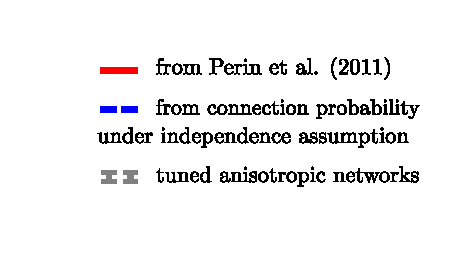
\includegraphics[width=0.5\textwidth]{%
      img/tuned_legend.pdf}   
  }%
  \vspace{-0.15cm}
  \caption{\textbf{Overrepresentation of reciprocal connections
      independent of } Comparison of occurrences of one- and
    bidirectionally connected neuron pairs in (gray) with profiles
    found by \textcite{Perin2011} (red), shows that overrepresentation of
    bidirectional pairs is distance-independent and not connected to
    anisotropy.  \textbf{A)} Overall connection probability in the
    adapted anisotropic networks was successfully tuned to reflect
    connection probability found by Perin et al. \textbf{B)-C)}
    Probabilities for a random neuron pair to display , 
    (\smtcite{875505b0})} %?? fix width issue!!
  \label{fig:perin_profiles}
\end{figure}



%%% Local Variables: 
%%% mode: latex
%%% TeX-master: "../dplths_document"
%%% End: 


% \begin{figure}[htp]
%   \centering
%     \begin{minipage}{.45\textwidth}

%         \begin{overpic}[width=\textwidth]{%
%             plots/6154302f.pdf}
%           \put(85.5,57.5){\small\textbf{A}}
%           % \put(12,5){\small\textbf{A}}
%         \end{overpic}
%         \vfill
%         \begin{overpic}[width=\textwidth]{%
%             plots/ef0e785d.pdf}
%           \put(90.5,58.2){\small\textbf{B}}
%         \end{overpic}

%       \end{minipage}
%       \hfill
%       \begin{minipage}{.45\textwidth}

%         \begin{overpic}[width=0.85\textwidth]{%
%             plots/bed7650b.pdf}
%         \end{overpic}
%        \vfill

%         \begin{overpic}[width=0.85\textwidth]{%
%             /users/hoffmann/research/connected_test.pdf}
%           % \put(90.5,58.2){\small\textbf{B}}
%         \end{overpic}
 
        
%       \end{minipage}
      
%   \vspace{-0.15cm}
%   \caption{ (\smtcite{6154302f}, \smtcite{ef0e785d})} %?? fix width issue!!
%   \label{fig:determine_side_length}
% \end{figure}


% \begin{figure}[htp]
%   \centering
%   \makebox{%
%     % \begin{overpic}[height=4.05cm]{%
%     %     plots/6154302f.pdf}
%     %   \put(85.5,57.5){\small\textbf{A}}
%     %   %\put(12,5){\small\textbf{A}}
%     % \end{overpic}
%     % \hfill
%     \begin{overpic}[height=4cm]{%
%         /users/hoffmann/research/connected_test.pdf}
%       % \put(90.5,58.2){\small\textbf{B}}
%     \end{overpic}
%   }%
%   \vspace{-0.15cm}
%   \caption{ (\smtcite{6154302f}, \smtcite{ef0e785d})} %?? fix width issue!!
%   \label{fig:tuned_width}
% \end{figure}